\documentclass[12pt, a4paper]{article}
\usepackage{graphicx}
\graphicspath{ {./images/} }
\usepackage{subcaption}


\title{Programozás alapjai 1 összefoglaló}
\author{Illyés Dávid}
\date{\today}
\begin{document}
\maketitle


\noindent\fbox{%
    \parbox{\textwidth}{
		Ez  a jegyzet nagyon hasonlóan van struktúrálva az előadás jegyzetekhez és fő célja, hogy olyan módon adja át a "A Programozás Alapjai 1" nevű tárgy anyagát, hogy az teljesen kezdők számára is könnyen megérthető és megtanulható legyen. 
    }
}


\section{előadás}

Ami itt kimarad:
1.előadás 2.fejezet - Alapfogalmak Imperatív

Algoritmus:
Gépiesen végrehajtható lépések véges sorozata, amely elvezet a megoldáshoz
Kódolás előtt három dologról kell meggyőződnünk:
helyes - tényleg azt csinálja amire szükségünk van
teljes minden elhetséges esetben elvégzi a dolgát
véges véges sok lépésben befejeződik

Algoritmusok leírása:

Algoritmusok leírási nyelvfüggetlen leírási módja a pszeudokód (álkód), ez természetes nyelven, de precÍzen megfogalmazott utasítássorozatot jelent.

 IDE JÖHET EGY EGYSZERŰ PÉLDA 

Algoritmusok grafikus ábrázolásának eszköze a folyamatábra.
Egy be- és kimenetű program folyamatábrája START és STOP  elemek között helyezkedik el

IDE KELL EGY ÁBRA 

A folyamatábra az alábbi elemekből épül fel


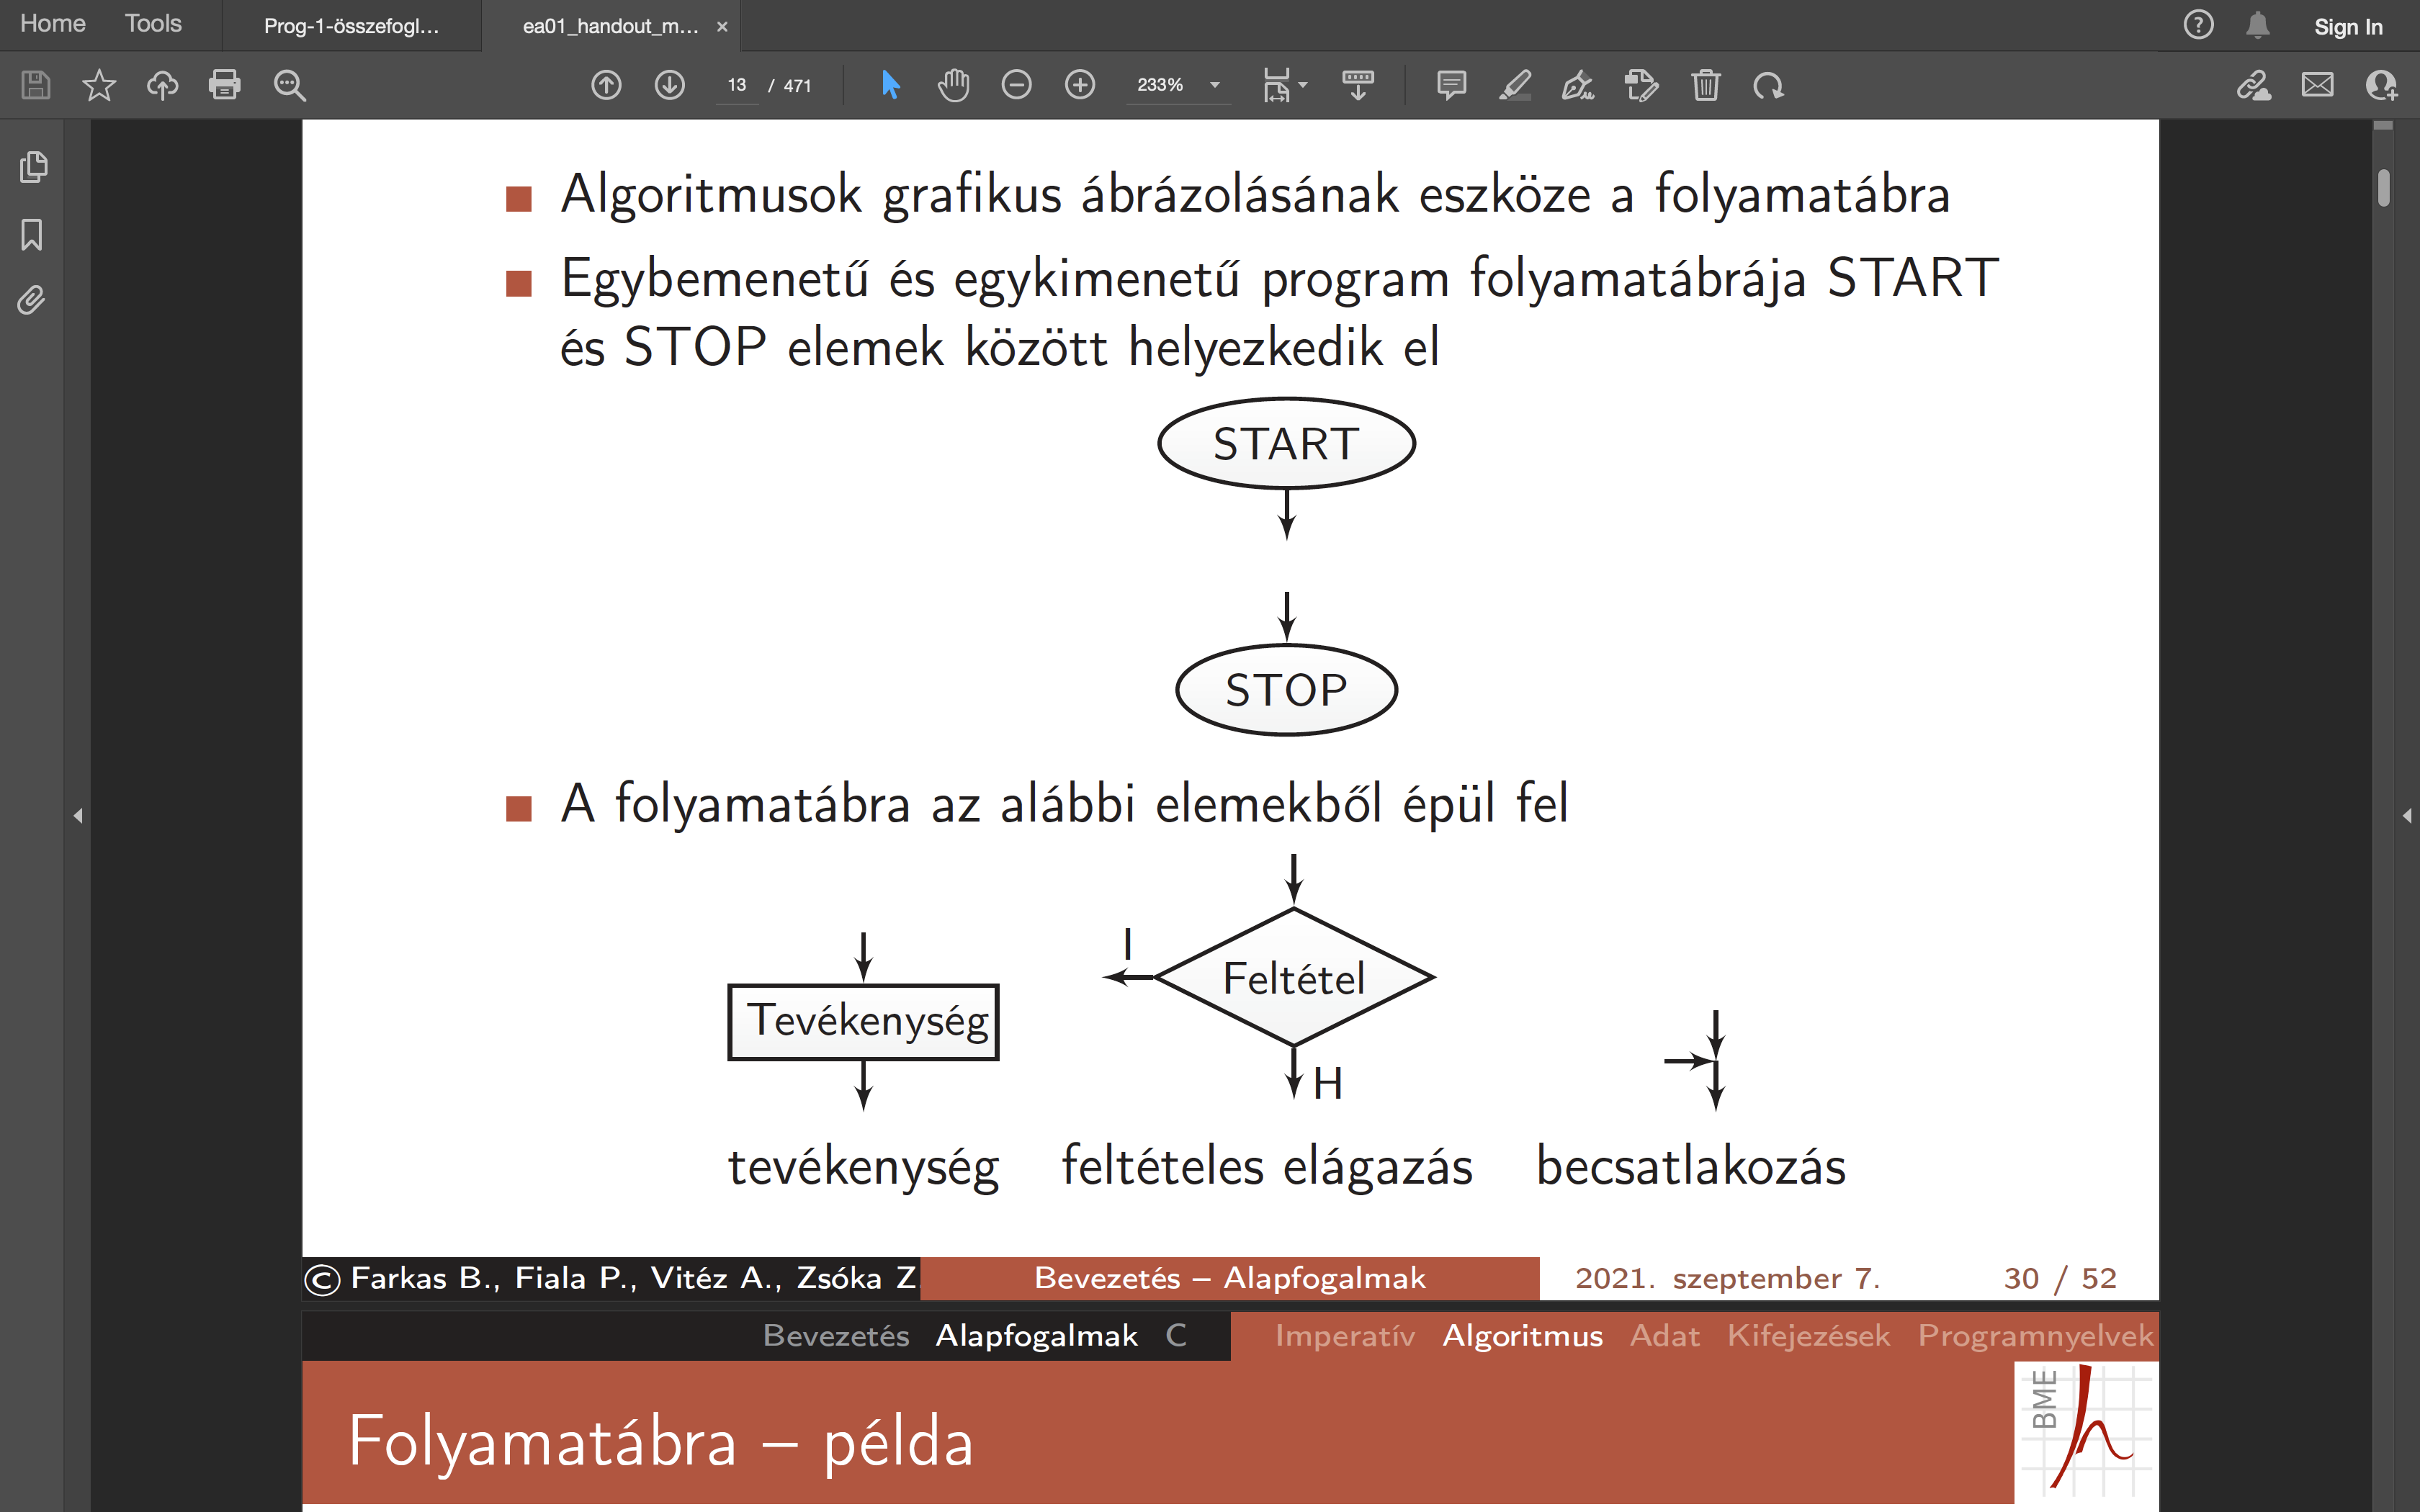
\includegraphics[scale= 0.2]{screen}
\caption{screen shot}


 IDE KELL EGY ÁBRA 

 IDE JÖHET EGY EGYSZERŰ PÉLDA 

 IDE JÖHET EGY EGYSZERŰ PÉLDA CIKLUSOKRA 

Az algoritmus adatokon, adatokkal dolgozik

Adat: Az adat minden, amit a külvilágból számítógépünkben leképezve tárolunk

Az adatnak van típusa (ez lehet szám, betű, szín) és értéke. Az adat típusa meghatározza az adat értékkészletét és az azon végezhető műveleteket.

 ADATTÍPUSOK FELSOROLÁSA TÁBLÁZATTAL  

XX Az adat lehet állandó vagy változó, az állandó (avagy konstans) adat értékkét nem lehet változtatni a változó létre XX

Változónak hívunk egy névvel ellátott értéket hordozó adattagot. Egy változónak kettő típusa van, a konstans "változó" és a változó változó

Ezekre egy egy példa:
Egy konstans változó lehet egy születési dátum, hiszen az egy adott pont az időben és nem lehet felülírni, pont ahogy egy konstans változót sem.

\section{előadás}

\begin{itemize}
	\item Szám:
	\begin{itemize}
		\item Értéke lehet: 0, -1, $e$, $\pi$
		\item Műveletek: összeadás, kivonás, összehasonlítás, rendezés
		\item Kiiratási kódja: %d
	\end{itemize}
	\item Betű:
	\begin{itemize}
		\item Értéke lehet: 0, -1, $e$, $\pi$
		\item Műveletek: összeadás, kivonás, összehasonlítás, rendezés
		\item Kiiratási kódja: %d
	\end{itemize}
	\item Logikai:
	\begin{itemize}
		\item Értéke lehet: 0, -1, $e$, $\pi$
		\item Műveletek: összeadás, kivonás, összehasonlítás, rendezés
		\item Kiiratási kódja: %d
	\end{itemize}
	\item Szín:
	\begin{itemize}
		\item Értéke lehet: 0, -1, $e$, $\pi$
		\item Műveletek: összeadás, kivonás, összehasonlítás, rendezés
		\item Kiiratási kódja: %d
	\end{itemize}
	\item Hőmérséklet:
	\begin{itemize}
		\item Értéke lehet: 0, -1, $e$, $\pi$
		\item Műveletek: összeadás, kivonás, összehasonlítás, rendezés
		\item Kiiratási kódja: %d
	\end{itemize}
\end{itemize}


\begin{itemize}

    \item [\textbf{TO-DO list:}]
    \item rendező algoritmusokat felsorolni

\end{itemize}

\end{document}



